\documentclass[runningheads]{llncs}

\usepackage[T1]{fontenc}
\usepackage[utf8]{inputenc}
\usepackage{booktabs}
\usepackage{hyperref}
\usepackage{microtype}
\usepackage{tabularx}

\usepackage{tikz}
\usetikzlibrary{arrows.meta,positioning,shapes.geometric}
\usepackage{xcolor}
\usepackage{pdfcomment}

\newcommand{\reviewcomment}[2]{%
  \pdfmarkupcomment[markup=Highlight,color={1 1 0}]{#1}{#2}%
}

\title{HCMO: A FAIR Ontology for Home-Cage Monitoring}
\titlerunning{HCMO: A FAIR Ontology for Home-Cage Monitoring}

\author{Cyril Gilbert\inst{1}\thanks{First and corresponding author.} \and
Gaoussou Sanou\inst{1} \and
Serge Sonfack Sounchio\inst{1} \and
Antoine Toffano\inst{1} \and
Pierre Larmande\inst{1} \and
Konstantin Todorov\inst{1}\thanks{Co-last author and corresponding author.} \and
Damien Huzard\inst{1}\thanks{Co-last author and corresponding author.}}
\authorrunning{C. Gilbert et al.}
\institute{Affiliations to be confirmed before submission.\\
\email{cyril.gilbert8@gmail.com,
konstantin.todorov@lirmm.fr, damien.huzard@gmail.com}}

\begin{document}
\maketitle

\begin{abstract}
Home-Cage Monitoring (HCM) systems observe laboratory animals continuously in their own cage, improving the contextual richness and reproducibility of preclinical data. Yet HCM systems are highly heterogeneous --- differing in sensors, measured variables, software, and output formats --- and their data are inseparable from a rich experimental context. This heterogeneity hinders comparison, reuse, and FAIR data sharing. We present HCMO, the Home-Cage Monitoring Ontology, which builds on earlier conceptual models of HCM and, to our knowledge, is the first machine-actionable ontology to represent HCM as an integrated experimental and data-acquisition system. HCMO is organised into five modules covering monitored enclosures, biological subjects, environmental context, observations and results, and technical acquisition. It is built around an explicit separation of sensor, observation, and result, preserving the chain from device to interpreted measurement. The published HCMO 0.3.0 release reuses BFO, IAO, the 2017 SOSA/SSN Recommendation, Schema.org, OWL-Time, and a reviewed SemTS 1.2.0 time-series segment pattern where their semantics fit. Provenance-backed state records and a pinned QUDT 3.4.0 quantity pattern are implemented; broader domain alignments remain future work. HCMO is delivered as a FAIR, tool-consumable package: modular sources, reproducibly generated distributions (Turtle/OWL/JSON-LD), SHACL shapes, competency-question queries, a JSON-LD context, persistent identifiers, an open licence, and documentation. We describe its design, evaluate it through competency questions and ontology-quality tooling, and discuss its uptake within the COST TEATIME community.

\keywords{ontology \and home-cage monitoring \and laboratory animals \and FAIR data \and SOSA/SSN \and 3Rs}
\end{abstract}


\begin{center}
\begin{minipage}{0.94\linewidth}
\small
\textbf{Resource type:} Ontology with SHACL shapes, SPARQL competency queries,
JSON-LD context, and example datasets\\
\textbf{License:} CC BY 4.0\\
\textbf{DOI:} \href{https://doi.org/10.5281/zenodo.22208202}{10.5281/zenodo.22208202}\\
\textbf{GitHub repository:} \url{https://github.com/dhuzard/HCMO}\\
\textbf{URL:} \url{https://w3id.org/hcmo/ontology/hcm}
\end{minipage}
\end{center}

\input{sections/01-introduction.tex}
\section{Related work}

\textbf{Home-Cage modelling.}
HCM is an active and rapidly growing field, with recent surveys describing available systems, sensing technologies, experimental applications, and do-it-yourself approaches \cite{kiryk2026,huzard2026tech,duarte2026diy}. In parallel, the HCM community has increasingly addressed the challenges created by heterogeneous data formats, incomplete metadata, and limited interoperability. Bains et al.\ \cite{bains2025} proposed a FAIR-compliant repository architecture for HCM data and metadata, emphasising standardised data structures, comprehensive metadata, and ontology-supported harmonisation as prerequisites for cross-system data reuse. This direction was subsequently developed further in work specifically addressing HCM data sharing and metadata \cite{forrest2026}, and connected to the broader ethical argument that preserving the scientific value and reusability of animal-derived data is itself part of responsible animal research \cite{petit2026wellfair}.

Importantly, semantic modelling of HCM also predates the present ontology. Within COST Action TEATIME, an Olog-based representation was developed to formalise what constitutes a home-cage monitoring system \cite{teatimeHCMDefinition,kiryk2026}. The work, led by Leonardo Restivo with contributions from Davor Virag and other TEATIME members, represented relationships among the animal, enclosure, hardware, software, sensors and actuators, behaviour and physiology, environmental provisions, duration of monitoring, and limited human interaction. The model was intended both to distinguish HCM systems from other experimental configurations and to identify key parameters that should be reported to describe an HCM experiment. This conceptual structure was also incorporated into the FAIR HCM repository work of Bains et al.\ \cite{bains2025}, providing an important precursor to the present work.

HCMO draws on this HCM-specific conceptual foundation while addressing a different level of formalisation. The TEATIME Olog provides a graphical, category-inspired conceptual model and explicitly adopts a simplified Olog representation rather than a deployable semantic-web ontology \cite{teatimeHCMDefinition}. Similarly, previous HCM data-sharing work establishes the need for standardised metadata, controlled terminology, and interoperable data structures, but does not provide a shared ontology capable of representing HCM experimental entities and their relationships in a machine-actionable form. HCMO addresses this formalisation gap through an explicit semantic model of the HCM acquisition chain—linking animal subjects, housing and environmental context, devices and sensors, observations, derived measurements, behaviours, and results—with formally defined entities and relations intended for annotation, validation, integration, and computational reuse across heterogeneous HCM platforms.


\textbf{Standards reused, not duplicated.} HCMO builds on W3C and community vocabularies. SOSA/SSN provides the sensor/observation/platform backbone \cite{sosa}; OWL-Time models temporal entities and intervals \cite{owltime}; QUDT provides quantity values and units \cite{qudt}; PROV captures provenance \cite{provo}; and BFO supplies an upper-ontology grounding for processes such as behaviour \cite{bfo}. SemTS provides a vocabulary for time-series segments and their dimensions \cite{semts}. HCMO reuses reviewed portions of these resources, contributing the HCM-specific concepts and relations that bind them.

\textbf{Adjacent biomedical and laboratory-animal ontologies.} Several resources cover neighbouring concerns. The Ontology for Biomedical Investigations (OBI) models investigations, protocols, instruments, materials, and data \cite{obi}; the Ontology of Laboratory Animal Medicine (OLAM) provides laboratory-animal terminology; and the Mouse Experimental Design Ontology (MEDO) standardises experimental-design descriptions, overlapping HCMO's housing/experimental-group notions. Reporting guidelines such as ARRIVE \cite{arrive} prescribe \emph{what} to report about in-vivo experiments but are not machine-readable ontologies. None of these model continuous in-cage acquisition; HCMO is complementary to them and can bridge to OBI and MEDO where appropriate.

The ISA framework provides a widely used investigation--study--assay exchange model \cite{isa}, while RO-Crate packages research data and contextual metadata as JSON-LD \cite{rocrate}. HCMO uses these as exchange targets in executable fixtures. This differs from asserting OWL mappings or complete formal conformance: the native ISA projections intentionally expose losses for HCM-specific housing, repeated-observation, and statistical-result structures.

\textbf{Ontology engineering.} Methodologically, HCMO follows an incremental, competency-question-driven process in the spirit of LOT \cite{lot2022} and SAMOD \cite{samod2017}, with requirements expressed as competency questions \cite{noy2001}. The current version was conceptualised graphically in diagrams.net and exported to OWL/Turtle with Chowlk \cite{chowlk2022}; LinkML was explored as an alternative serialisation \cite{linkml2021}. Documentation is produced with WIDOCO \cite{widoco2017}, and quality is assessed with OOPS! \cite{oops2012} and, for FAIRness, FOOPS! \cite{foops}, complemented by reasoning and SHACL validation \cite{gangemi2006}. Positioned this way, HCMO is the first ontology dedicated to HCM, designed to interoperate with --- rather than replace --- the surrounding standards and biomedical ontologies.

\section{Requirements and competency questions}
\textbf{Stakeholders and use cases.} HCMO is intended for several roles: researchers comparing or aggregating behavioural and physiological data across studies and laboratories; facility managers and welfare committees auditing housing and husbandry; data engineers ingesting heterogeneous device exports; and, in the longer term, downstream AI consumers querying the resulting knowledge graph. These roles share one need --- to interpret a measurement together with the full context of its production.

\textbf{Requirements from domain analysis.} Analysis of the HCM domain \cite{kiryk2026,huzard2026tech,forrest2026} yields the following requirements, which drive the model (forward references to \S{}4):

\begin{itemize}
\item \textbf{R1 --- Context-complete observations.} Every observation must record the
concerned subject, the observed property, the time, the procedure, and, where available, the result, so that no measurement is stranded without context.

\item \textbf{R2 --- Separation of device, observation, and result.} A sensor (a technical
device), an observation (the measurement event in context), and a result (the produced value/interpretation) must be modelled distinctly, preserving the chain \emph{device $\rightarrow$ observation $\rightarrow$ measurement $\rightarrow$ interpretation}. HCM outputs are often signals later transformed by software into inferred behaviours.

\item \textbf{R3 --- Temporal housing assignment.} Membership of an animal in an enclosure is
time-bounded, not permanent, and must be represented as an assignment over an interval, linked to experimental groups and study factors.

\item \textbf{R4 --- Environment as interpretable context.} Enclosure dimensions, enrichment,
light cycles, and measurable conditions (temperature, humidity, gas, light) must be representable, distinguishing a \emph{property} from the \emph{values} observed for it.

\item \textbf{R5 --- Technical provenance.} Hardware, sensors, software, and their
organisation of data into time series/segments must be captured without conflating technical provenance with biological interpretation.

\item \textbf{R6 --- Rich, machine-readable metadata.} Species, strain, sex, age, housing,
enrichment, device configuration, sampling rate, software, and protocol must be first-class, supporting FAIR reuse \cite{fair,forrest2026}.

\item \textbf{R7 --- Standards reuse and interoperability.} Where a suitable standard
exists, it must be reused rather than re-minted. Candidate standards include SOSA/SSN, OWL-Time, BFO/IAO, PROV-O, and reviewed quantity/unit vocabularies; each mapping strength must be justified separately.

\item \textbf{R8 --- Data-quality checking.} The model must support consistency and
completeness checks (e.g. a numeric value without a unit, an animal not assigned to an enclosure over an interval).

\end{itemize}

\textbf{Competency questions.} Requirements are operationalised as executable SPARQL questions \cite{noy2001,lot2022}. The release index contains eleven questions. They retrieve assignments by enclosure and at a reference time; missing enclosure dimensions; environment specifications paired with observed QUDT quantities; time-bounded operational and calibration evidence; husbandry provisioning gaps; sensor-captured properties; observations lasting at least 24 hours under a stated condition; and three ISA/STATO provenance paths. Complete expected bindings are versioned with the queries, including the intentionally empty missing-dimensions answer. Section 6 reports their exact results. Five additional queries exercise the isolated 2 $\times$ 2 round-trip fixture for housing history, factor assignments, repeated observations, statistical result/file-fragment separation, and the Source-to-Sample derivation.

\section{Resource description}
HCMO uses the persistent ontology IRI \nolinkurl{https://w3id.org/hcmo/ontology/hcm} and the stable term namespace \nolinkurl{https://w3id.org/hcmo/ontology/hcm#}. Domain-specific terms use four sub-namespaces beneath the same base: \nolinkurl{hcm/bio#}, \nolinkurl{hcm/env#}, \nolinkurl{hcm/obs#}, and \nolinkurl{hcm/tech#}. Published IRIs are not renamed when terminology changes; obsolete IRIs are retained in a compatibility module with deprecation and replacement metadata where a defensible replacement exists.

\textbf{Modular organisation.} The paper-matching HCMO candidate is authored as five active modules. The minimal core centres on \nolinkurl{hcm:Enclosure}, \nolinkurl{hcm:MonitoredEnclosure}, enclosure dimensions, enrichment, and stable housing relations. The bio module represents subjects, experimental groups, housing assignments, and study factors. The env module represents environmental profiles, light cycles, gas profiles, measurement specifications, and environmental properties. The obs module owns SOSA-style observations and their categorical, quantitative, behavioral, and tabular results. The tech module represents sensors, actuators, hardware, software, and time-series resources. A sixth, migration-only module preserves deprecated HCMO 0.0.1 IRIs but is not a source of terms for new data.

This organisation preserves two boundaries that are important for HCM data. First, housing context is not reduced to the animal: a housing assignment is an explicit record linking a subject or group to an enclosure. Second, a physical sensor, the observation it performs, and the result it produces are separate entities. For example, \nolinkurl{hcm-tech:Sensor} is linked to a monitored enclosure, captures a \nolinkurl{sosa:ObservableProperty}, and may make a \nolinkurl{sosa:Observation}; the observation then identifies its feature of interest and result using SOSA relations. This supports provenance-sensitive queries without treating a device, event, and data value as the same thing.

Environmental profiles, measurement specifications, and observations likewise use different relations: a profile composes specifications, each specification identifies the property and optional target quantity, and each observation uses the SOSA observed-property/result pattern. Housing membership is derived from time-bounded assignments at a stated time. Operational and calibration states are time-bounded records generated by explicit PROV activities rather than timeless booleans.

\textbf{Standards reuse.} Physical subjects, enclosures, enrichments, sensors, actuators, hardware, and experimental groups are exposed under BFO material entity in the default end-user hierarchy. Records, specifications, profiles, software, and observation-result artifacts use the IAO information-content anchor. A separate optional developer profile restores BFO's source-faithful intermediate hierarchy and the more precise object-aggregate classification of experimental groups. Sensors, actuators, observations, results, and observed properties reuse SOSA classes and relations, and \nolinkurl{hcm-tech:captures} is explicitly a subproperty of \nolinkurl{sosa:observes}. Schema.org supplies contributor and place exchange types. The example ABox uses OWL-Time intervals and the duration competency query consumes this representation. These are selective references, not claims that HCMO imports or reproduces the full external ontologies.

Numeric dimensions, sampling rates, environmental targets, and observation results use the pinned QUDT 3.4.0 \nolinkurl{QuantityValue}, \nolinkurl{numericValue}, and \nolinkurl{hasUnit} pattern \cite{qudt}. HCMO role properties state what each quantity describes. This is selective reuse of the checksummed schema and unit vocabulary, not a claim of full QUDT conformance.

\textbf{Claim strength.} We distinguish implemented semantic reuse or alignment, validated interoperability evidence, and formal profile conformance. Implemented alignment requires canonical versioned terms, reviewed semantic fit, and a normative role in HCMO; its assertion strength is stated per term and never generalized to a whole vocabulary. Interoperability evidence means that a pinned mixed-vocabulary example is validated and queried, but does not by itself establish ontology mappings or complete round trips. Formal conformance is reserved for a declared version and scope in which every applicable normative profile requirement has been tested. ``Provisional'' identifies work that has not yet qualified as implemented alignment; it is not a conformance level.

HCMO normatively follows the 2017 SOSA/SSN Recommendation \cite{sosa}, pinned to an immutable copy of the 2017 ontology artifact. Environmental and sensor-captured properties use \nolinkurl{sosa:ObservableProperty}; terms introduced by the developing later edition are not mixed into this release. HCMO also selectively reuses canonical unversioned SemTS 1.2.0 terms \cite{semts}: a location result table is a \nolinkurl{semts:TimeSeriesSegment} whose dimensions may be linked with \nolinkurl{semts:segmentDimension} to \nolinkurl{semts:DataDimension}. The earlier observation dimension restriction and knowledge-generation-specific \nolinkurl{semts:generated} relation were removed after semantic review. A pinned example-level evidence slice now uses PROV-O, specific OBI and STATO types, and ISA/Bioschemas exchange terms in one acyclic workflow \cite{isa,rocrate}. This is validated interoperability evidence, not an HCMO class mapping or a claim of formal ISA RO-Crate conformance. A second generated 2 $\times$ 2 fixture preserves animal identity, time-bounded housing, Source/Sample roles, repeated observations, factor/group structure, and separate STATO results and file fragments across a graph-isomorphic HCMO RDF/extended ISA RO-Crate pair. RO-Crate 1.2 and ISA-specific required validator rules pass. Formal ISA conformance remains deferred because the draft has no permanent profile URI and its validator currently disagrees about the base RO-Crate edition. ISA-JSON and ISA-Tab are controlled-loss projections. Their executable native overlap, tested with pinned \nolinkurl{isatools} 0.14.3, preserves a distinct animal Source, a real tissue Sample, their collection process and their HCMO identifiers through a JSON--Tab--JSON cycle. Housing, direct whole-animal recording, source-bound factor assignments, explicit groups, repeated observations, and semantic STATO/file-fragment links remain declared losses rather than being represented with fabricated Sample proxies. Broader logical mappings and integration remain separately reviewed work.

\textbf{Distribution and application support.} The authored modules are merged deterministically into Turtle, RDF/XML, and JSON-LD distributions. A generated \nolinkurl{profile.json} provides a flat term inventory for synchronization layers and interfaces, while \nolinkurl{ontology/context.jsonld} supports JSON-LD applications. \nolinkurl{hcmo.yaml} is the stable machine-readable contract that identifies the module order, generated artifacts, shapes, examples, and competency-query index.

The active source inventory contains 33 classes and 69 non-deprecated object or datatype properties. The generated release additionally contains deprecated compatibility terms and directly referenced external vocabulary terms. A signed class audit and property audit record the asserted semantics, restrictions, inference consequences, current evidence, and unresolved decisions without turning review notes into unattended ontology rewrites.

\begin{figure*}[t]
\centering
\resizebox{\textwidth}{!}{%
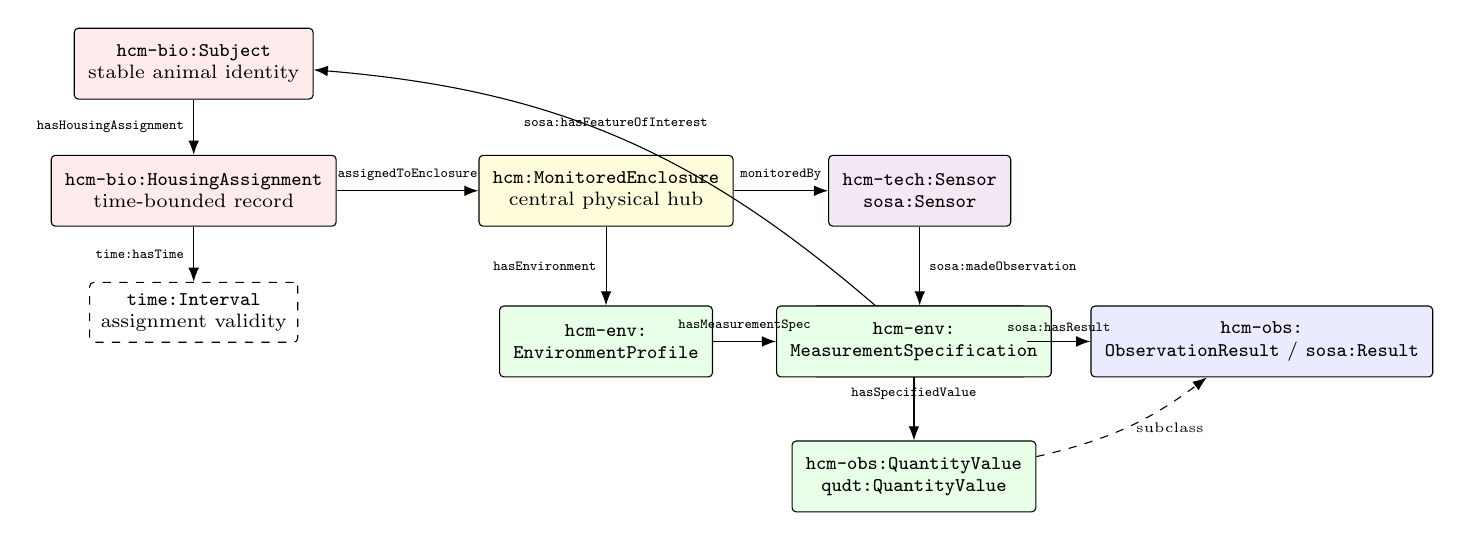
\begin{tikzpicture}[
  node distance=7mm and 9mm,
  entity/.style={draw, rounded corners=1.5pt, align=center, minimum height=9mm, font=\scriptsize, inner xsep=5pt},
  rel/.style={-{Latex[length=1.8mm]}, font=\tiny},
  evidence/.style={draw, dashed, rounded corners=1.5pt, align=center, font=\scriptsize, inner sep=4pt}
]
\node[entity, fill=yellow!14] (cage) {\texttt{hcm:MonitoredEnclosure}\\central physical hub};
\node[entity, fill=red!8, left=18mm of cage] (assignment) {\texttt{hcm-bio:HousingAssignment}\\time-bounded record};
\node[entity, fill=red!8, above=of assignment] (subject) {\texttt{hcm-bio:Subject}\\stable animal identity};
\node[entity, fill=violet!9, right=12mm of cage] (sensor) {\texttt{hcm-tech:Sensor}\\\texttt{sosa:Sensor}};
\node[entity, fill=blue!8, below=10mm of sensor] (observation) {HCMO observation\\\texttt{sosa:Observation}};
\node[entity, fill=blue!8, right=8mm of observation] (result) {\texttt{hcm-obs:}\\\texttt{ObservationResult} / \texttt{sosa:Result}};
\node[entity, fill=green!9, below=10mm of cage] (profile) {\texttt{hcm-env:}\\\texttt{EnvironmentProfile}};
\node[entity, fill=green!9, right=8mm of profile] (spec) {\texttt{hcm-env:}\\\texttt{MeasurementSpecification}};
\node[entity, fill=green!9, below=8mm of spec] (quantity) {\texttt{hcm-obs:QuantityValue}\\\texttt{qudt:QuantityValue}};
\node[evidence, below=of assignment] (time) {\texttt{time:Interval}\\assignment validity};

\draw[rel] (subject) -- node[left]{\texttt{hasHousingAssignment}} (assignment);
\draw[rel] (assignment) -- node[above]{\texttt{assignedToEnclosure}} (cage);
\draw[rel] (assignment) -- node[left]{\texttt{time:hasTime}} (time);
\draw[rel] (cage) -- node[above]{\texttt{monitoredBy}} (sensor);
\draw[rel] (sensor) -- node[right]{\texttt{sosa:madeObservation}} (observation);
\draw[rel] (observation) -- node[above]{\texttt{sosa:hasResult}} (result);
\draw[rel, dashed] (quantity) to[bend right=12] node[right]{subclass} (result);
\draw[rel] (observation) to[bend right=18] node[above]{\texttt{sosa:hasFeatureOfInterest}} (subject);
\draw[rel] (cage) -- node[left]{\texttt{hasEnvironment}} (profile);
\draw[rel] (profile) -- node[above]{\texttt{hasMeasurementSpec}} (spec);
\draw[rel] (spec) -- node[above]{\texttt{hasSpecifiedValue}} (quantity);
\end{tikzpicture}
}
\caption{The five-module HCMO model preserves animal identity, temporal housing,
environmental specifications, sensing events, and results as distinct entities.}
\label{fig:domain-model}
\end{figure*}


\section{Engineering, availability, and sustainability}
HCMO is released not as a single file but as a \textbf{tool-consumable package} designed so that downstream tools can resolve every component programmatically.

\textbf{Release manifest as a stable contract.} A machine-readable manifest (\nolinkurl{hcmo.yaml}) declares the ontology's identity (name, version, namespace, prefix, ontology and version IRIs), the ordered list of source modules, the generated distributions, the SHACL shapes, the competency-question index, and the example datasets. Its \emph{shape} is treated as an API and kept stable across releases, so a consumer (e.g. a synchronisation or question-answering layer) can discover paths from the manifest rather than hard-coding them.

\textbf{Modular sources and reproducible distributions.} The ontology is authored as five modular Turtle sources (\emph{core/bio/env/obs/tech}) plus a migration-only compatibility module. A build step merges them into a canonical, sorted serialisation, producing byte-identical output on re-run so that version-control diffs stay clean. The merged graph is published in three syntaxes --- Turtle, RDF/XML (OWL), and JSON-LD --- together with a flat term inventory (\nolinkurl{profile.json}: IRIs, labels, comments, and counts) intended for sync layers and user interfaces. Everything under the distribution directory is generated; only the modules are edited by hand. The manifest still identifies version 0.2.0, but the paper-matching graph contains 24 later commits, including the ISA/STATO, SemTS/SOSA, temporal-state, and QUDT work. A new version and tag must therefore be assigned before submission; the tagged 0.2.0 artifact is not presented as the evaluated paper release.

\textbf{Continuous validation.} A validation step parses every Turtle file, runs the SHACL shapes with RDFS entailment against isolated positive and intentionally invalid example ABoxes, and executes each competency-question query against the ontology plus positive examples. Complete expected answer rows make changed bindings, multiplicities, values, and unexamined empty results a validation failure even when the row count is unchanged. The same check runs in CI as the pull-request gate, and a tag-triggered workflow attaches the distributions to a GitHub release. This makes the resource's quality claims reproducible by any third party.

\textbf{Availability (FAIR).} HCMO targets the Resources-Track availability criteria \cite{fair}:

\begin{itemize}
\item \emph{Findable / Interoperable identification.} The ontology and its terms are
identified by a persistent \nolinkurl{w3id.org} IRI (\nolinkurl{https://w3id.org/hcmo/ontology/hcm#}, which dereferences via HTTP 303 content negotiation to the documentation); the resource is archived on Zenodo with a DOI.

\item \emph{Accessible.} Sources and distributions are openly available from the public
Git repository and the Zenodo deposit (download), with HTML documentation served via GitHub Pages. A public \textbf{SPARQL endpoint} will be provided for live querying. \emph{[pending: host the endpoint --- T6b.]}

\item \emph{Interoperable.} The current model reuses BFO \cite{bfo}, IAO, and SOSA/SSN
\cite{sosa} anchors, with Schema.org; example data reuse OWL-Time \cite{owltime}. SOSA is pinned to the 2017 Recommendation and uses \nolinkurl{sosa:ObservableProperty}. Canonical SemTS 1.2.0 segment and dimension terms are selectively reused for location result tables. A pinned example-level evidence slice uses PROV-O \cite{provo}, OBI, STATO, and ISA/Bioschemas without asserting HCMO class mappings or formal ISA RO-Crate conformance. The release also uses a pinned QUDT 3.4.0 quantity-value pattern for dimensions, sampling rates, specifications, and measured results. Broader vocabulary mappings remain future alignment work. A JSON-LD context is shipped for application developers exchanging data.

\item \emph{Reusable.} The resource is licensed CC BY 4.0, carries provenance on the
ontology header (creators with ORCIDs, version IRI), and provides a canonical citation (\nolinkurl{CITATION.cff}) plus a DOI.

\end{itemize}

Human- and machine-readable documentation is generated from the merged graph with WIDOCO \cite{widoco2017} (overview, term cross-reference, namespace declarations, a WebVOWL diagram, and provenance), published at the project's documentation site.

\textbf{Sustainability and governance.} HCMO is \textbf{lab-maintained} by the Huzard group: development is on GitHub with public issues and pull requests, versioning follows SemVer mirrored by \nolinkurl{owl:versionIRI}, and terms are deprecated rather than deleted or re-minted to protect external references. The COST \textbf{TEATIME} network serves as the community feedback channel grounding the model in real domain needs. A FAIR self-assessment (F/A/I/R) is given in the appendix (see \nolinkurl{metadata/resource-metadata.md}).

\begin{figure}[t]
\centering
\resizebox{\linewidth}{!}{%
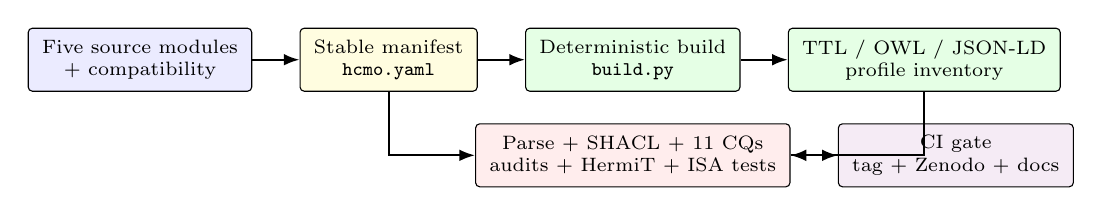
\begin{tikzpicture}[
  node distance=4mm and 6mm,
  box/.style={draw, rounded corners=1.5pt, align=center, minimum height=8mm, font=\scriptsize, inner xsep=5pt},
  flow/.style={-{Latex[length=2mm]}, thick}
]
\node[box, fill=blue!8] (src) {Five source modules\\+ compatibility};
\node[box, fill=yellow!12, right=of src] (manifest) {Stable manifest\\\texttt{hcmo.yaml}};
\node[box, fill=green!10, right=of manifest] (build) {Deterministic build\\\texttt{build.py}};
\node[box, fill=green!10, right=of build] (dist) {TTL / OWL / JSON-LD\\profile inventory};
\node[box, fill=red!7, below=of build] (validate) {Parse + SHACL + 11 CQs\\audits + HermiT + ISA tests};
\node[box, fill=violet!8, right=of validate] (release) {CI gate\\tag + Zenodo + docs};
\draw[flow] (src) -- (manifest);
\draw[flow] (manifest) -- (build);
\draw[flow] (build) -- (dist);
\draw[flow] (dist) |- (validate);
\draw[flow] (validate) -- (release);
\draw[flow] (manifest) |- (validate);
\end{tikzpicture}
}
\caption{HCMO's manifest-driven, reproducible build and validation pipeline.}
\label{fig:pipeline}
\end{figure}


\section{Evaluation}
HCMO is evaluated at four complementary levels: common ontology pitfalls and FAIR metadata, OWL consistency, instance-data validation, and executable competency questions. Reports and raw outputs are retained in the repository so that historical scores are not silently attributed to a later artifact.

\textbf{Pitfalls and FAIRness.} Historical scans of the clean-v2 precursor are kept as remediation evidence but are not attributed to the current graph. On 15 August 2026, OOPS! was rerun directly on the candidate RDF/XML distribution. It reported P04, P08, P10, P13, P22, P34, and P35. The important P10 finding is the scanner's ontology-wide missing-disjointness heuristic and names no affected pair. P34 and P35 concern reused SOSA, SemTS, QUDT, Schema.org, and PROV terms whose authoritative declarations are covered by HCMO's pinned external-vocabulary contract rather than copied into the merged graph. The minor P04, P08, and P22 findings likewise concern reused BFO or external terms. P13 marks 32 properties as lacking inverse declarations; candidate inverses are not asserted without definition-level evidence because doing so would create false entailments merely to satisfy a scanner.

FOOPS! was rerun by uploading the canonical candidate RDF/XML distribution and scored 1.0. All ontology metadata, licensing, provenance, resolvability, vocabulary-reuse, label, and definition tests passed. A separate deployment check found that the public PURL still served the older 1,252-triple graph rather than the 1,397-triple candidate, so the perfect candidate-file score is not misreported as a score for the currently deployed representation. Raw outputs and term-level triage are archived in \nolinkurl{docs/paper/evaluation/CANDIDATE-OOPS-FOOPS-2026-08-15.md}. Both scanners will be rerun after the candidate receives its final version IRI, tag, and PURL target.

\textbf{Logical consistency.} The canonical RDF/XML artifact was rebuilt and checksummed on 15 August 2026. \nolinkurl{dist/hcmo.owl} contains 1,397 RDF triples; the generated profile contains 60 declared release classes, 68 object properties, and 75 datatype properties, including compatibility and directly referenced external terms. HermiT loaded 65 classes and reported zero inconsistent classes. The pre-check also found no active \nolinkurl{UNKNOWN:} IRI and no property declared as both object and datatype. The exact checksum, environment, output, and triage are archived in \nolinkurl{docs/paper/evaluation/POST-PR24-26-REVIEW-2026-08-15.md}.

\textbf{SHACL validation.} The validator supplies the canonical ontology as a separate ontology graph and enables RDFS entailment when validating each example. This allows domain, range, and subclass consequences to select the same \nolinkurl{sh:targetClass} constraints as explicit types. Three positive examples conform, while two edge-case examples produce their reviewed violations. One negative fixture deliberately omits explicit \nolinkurl{rdf:type}: it conforms when validated without the ontology, then fails when ontology-aware inference selects the intended targets. This differential test guards the validator's entailment contract while keeping profile requiredness in SHACL rather than translating it into OWL existential semantics. A separate ISA/STATO evidence shape validates the pinned workflow boundary; an injected process/data cycle is required to fail.

The accepted round-trip fixture contains a 2 $\times$ 2 treatment-by-enrichment design with eight individually housed animals, 56 repeated dark-phase activity observations, non-overlapping re-housing, an actual derived tissue Sample, and separate fitted-model, estimate, confidence-interval, p-value, File, and file-fragment entities. Canonical HCMO RDF and extended ISA RO-Crate JSON-LD are graph-isomorphic at 1,539 triples. Dark-phase outcomes use phenomenon intervals, and the re-housed animal's observations resolve to its new enclosure through the authoritative assignment. The declared mixed model is executed against the generated CSV with pinned numerical dependencies; the model serialization and the active-versus-vehicle contrast at standard enrichment use distinct exact row fragments. Dedicated shapes and injected probes reject overlapping, orphaned, reversed, or incompletely generated housing assignments; generated replacement animals; observation/ housing mismatch; group/factor disagreement; and fabricated ISA assignment results.

\textbf{Competency questions.} Eleven SPARQL queries run over the ontology plus all positive examples. Negative fixtures are isolated from the query graph. The validator checks both query-index completeness and the complete expected answer rows, including bindings, unbound values, and multiplicity:

\begin{table}[t]
\centering
\small
\begin{tabularx}{\linewidth}{@{}Xr@{}}
\toprule
Competency question & Exact answers \\
\midrule
subjects assigned by monitored enclosure & 3 \\
ISA factor/group assignment & 1 \\
ISA raw-file recording provenance & 1 \\
OBI transformation and STATO result provenance & 1 \\
enclosures missing dimension records & 0 \\
environmental specification and observation quantities & 1 \\
current housing at the reviewed reference time & 1 \\
operational and calibration evidence at the reviewed time & 1 \\
housed subjects needing provisioning & 3 \\
properties captured by enclosure sensors & 4 \\
systems with observations lasting at least 24 hours under a condition & 1 \\
\bottomrule
\end{tabularx}
\end{table}

The zero-row dimensions query is intentional: it verifies absence of missing records in the positive fixture rather than being accepted as an unexamined empty result. The three ISA/STATO questions establish a narrow executable evidence slice; they do not establish HCMO class mappings or formal ISA RO-Crate conformance.

Five additional exact-answer questions run against the isolated round-trip fixture: nine housing-history rows, eight authoritative subject/group/factor rows, eight per-animal repeated-observation counts, four statistical-result/ file-fragment rows including exact values and meaning links, and one Source-to-derived-Sample row. \nolinkurl{roc-validator} 0.11.3 passes all RO-Crate 1.2 required rules and all ISA-specific required rules. Its full inherited ISA run has one isolated upstream conflict: the embedded ISA profile requires RO-Crate 1.1 although its minimal ISA fixture uses the 1.2 context. We report this as interoperability evidence, not formal conformance. Separately, pinned \nolinkurl{isatools} 0.14.3 validates an executable native projection and round trip for the genuine Source-to-Sample collection. Exact HCMO identifiers survive as ISA comments. The test deliberately excludes non-native housing, direct whole-animal assay, source-bound factor assignment, group, repeated-observation, and semantic-result/file-fragment structures and checks their loss manifests.

\begin{figure}[t]
\centering
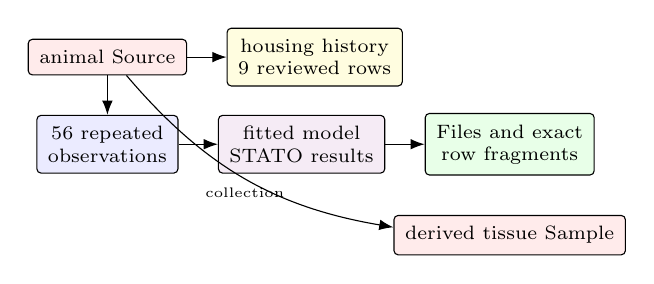
\begin{tikzpicture}[
  node distance=5mm and 5mm,
  box/.style={draw, rounded corners=1.5pt, align=center, font=\scriptsize, inner sep=4pt},
  flow/.style={-{Latex[length=1.8mm]}, font=\tiny}
]
\node[box, fill=red!8] (animal) {animal Source};
\node[box, fill=yellow!12, right=of animal] (housing) {housing history\\9 reviewed rows};
\node[box, fill=blue!8, below=of animal] (obs) {56 repeated\\observations};
\node[box, fill=violet!8, right=of obs] (model) {fitted model\\STATO results};
\node[box, fill=green!9, right=of model] (files) {Files and exact\\row fragments};
\node[box, fill=red!8, below=of files] (sample) {derived tissue Sample};
\draw[flow] (animal) -- (housing);
\draw[flow] (animal) -- (obs);
\draw[flow] (obs) -- (model);
\draw[flow] (model) -- (files);
\draw[flow] (animal) to[bend right=20] node[below]{collection} (sample);
\end{tikzpicture}
\caption{Executable 2 $\times$ 2 fixture used to test identity, housing,
repeated observations, statistical semantics, and ISA projection boundaries.}
\label{fig:roundtrip}
\end{figure}


\section{Impact, use cases, and outlook}
\textbf{Why HCMO matters.} HCM datasets are often distributed as system-specific exports in which measurements are weakly linked—or not linked at all—to the biological subject, enclosure, environmental context, acquisition device, software, and experimental protocol \cite{bains2025,forrest2026,petit2026wellfair}. HCMO provides a shared, machine-actionable semantic model for representing these dependencies consistently. By making the provenance and experimental context of each measurement explicit, HCMO can support dataset discovery, cross-system comparison, integration, and reuse, provided that datasets are mapped to the ontology and exposed with appropriate identifiers and metadata. It thus provides a foundation for transforming otherwise siloed records into interoperable and queryable knowledge. In animal research, where data constitute the durable output of an experiment, preserving their context and interpretability also has ethical relevance: it can reduce avoidable duplication, enable secondary analyses, and increase the scientific value obtained from each animal. HCMO may therefore support the Reduction and Refinement principles of the 3Rs, consistent with the WellFAIR view that data quality and animal welfare are interconnected \cite{petit2026wellfair}.

\textbf{Reasoning and data quality.}
Beyond semantic organisation, HCMO provides a formal basis for automated validation and reasoning. At an immediately applicable level, HCMO and its associated SHACL shapes can identify missing or inconsistent metadata during ingestion---for example, an observation with a numerical value but no unit, or an animal without a valid enclosure assignment during the observation interval. Such checks make data-quality requirements explicit and executable rather than leaving them to manual inspection.

At a second level, HCMO can provide an explicit semantic scaffold for AI-supported analysis. When incorporated into retrieval, query-generation, or agentic workflows, the ontology can specify admissible entity types and relations, as well as the contextual information required to interpret a measurement. The ontology does not, by itself, prevent erroneous inference. Rather, it provides constraints that can be enforced through schema validation, ontology-aware retrieval, and type-constrained query generation, thereby making downstream analyses more controlled, traceable, and interpretable than approaches based on statistical associations alone.

\textbf{Potential uses (outlook).}
HCMO is designed to underpin further tooling that is neither implemented nor evaluated as a contribution of the present work:
\begin{itemize}
    \item \emph{Knowledge-graph question answering.}
    HCMO can provide the schema for an HCM knowledge graph queried using natural language. A user question could be translated into a formal query, checked against the ontology, executed over the graph, and returned with the relevant results and provenance. Implementing this workflow would require reliable natural-language-to-query translation and validation. Related work demonstrates how knowledge graphs and graph embeddings can support structured retrieval, inference, and discovery, including in biomedical applications \cite{sanou2026,bian2025}. The same graph could support symbolic reasoning or graph-learning methods that exploit HCMO's class hierarchy and explicitly typed relations \cite{butz}.

    \item \emph{Assisted authoring.}
    User-facing forms could be generated from the ontology and its SHACL constraints to guide researchers through mandatory and recommended fields. The resulting HCMO-conformant RDF instance data, or ABoxes, could be validated before export or deposition, allowing biologists to produce well-structured data without needing to work directly with RDF, OWL, or SHACL.

    \item \emph{Vendor-data mapping.}
    Mapping components could transform proprietary device exports into HCMO while preserving the original values, identifiers, and provenance. HCMO would thereby provide a common semantic layer for cross-system comparison without requiring vendors or laboratories to adopt a single acquisition format.

\end{itemize}

\textbf{Adoption path.} Development is grounded with a network of preclinical and HCM experts, that initiated with COST-\textbf{TEATIME} action (CA20135), which provides domain feedback and a route to real datasets for validation and uptake. This community anchoring is intended to drive adoption beyond a single laboratory and to keep the model aligned with evolving HCM practices and technologies.

\section{Conclusion and future work}
We presented HCMO, the first ontology to model Home-Cage Monitoring as an integrated system spanning the animal subject, its housing, the environment, and the technical acquisition chain. HCMO captures HCM data together with the experimental context that makes them interpretable, keeps sensor, observation, and result distinct, and reuses selected terms from BFO, IAO, SOSA/SSN, Schema.org, OWL-Time, and QUDT rather than duplicating them. HCMO pins SOSA to the 2017 Recommendation and selectively reuses canonical SemTS 1.2.0 segment terms. A pinned instance-level ISA/Bioschemas, PROV-O, OBI, and STATO evidence slice demonstrates one acyclic recording-to-statistical-result workflow without claiming HCMO class mappings or formal ISA conformance. A generated 2 $\times$ 2 round-trip fixture further preserves animal identity, housing history, factors, groups, repeated observations, and separate semantic statistical results and their representing file fragments in HCMO RDF and an extended ISA RO-Crate. A narrower native ISA-JSON/ISA-Tab test preserves the real animal-Source-to-tissue-Sample collection without fabricating an animal Sample; all excluded HCMO/STATO structures are reported as controlled losses. HCMO is delivered as a FAIR, tool-consumable resource --- modular sources, reproducible distributions, SHACL shapes, competency-question queries, a JSON-LD context, persistent identifiers, an open licence, and documentation --- and is grounded in the COST TEATIME community.

\textbf{Limitations.} HCMO is still an early and evolving resource. Some conceptual boundaries are being stabilised, most notably between raw data, processed measurement, interpreted observation, and biological result, where the same information can be viewed at several levels. The diversity of HCM systems makes a single model that is both broad enough to be reusable and precise enough to describe individual experiments an ongoing balance. Alignment to external vocabularies is deliberately partial in this version. The factorial and mixed-model resources are interoperability fixtures, not a general HCMO statistics hierarchy. Complex pathologies and AI models on the data remain outside the stabilised core.

\textbf{Future work.} Planned directions include expert review of definitions and axioms identified by the class and property audits; systematic alignment decisions (reuse as-is vs specialise vs keep HCMO-specific) and bridge modules to adjacent ontologies (e.g. OBI, PROV-O, STATO, MEDO) and to taxa/anatomy/device vocabularies; extending the current selective QUDT pattern to additional quantity roles where justified; populating the ontology with real datasets via the TEATIME network and publishing the corresponding SPARQL queries; and supporting the downstream uses outlined in \S{}7. Through these steps, HCMO aims to become a community reference that improves the annotation, comparison, and reuse of HCM data across laboratories.


\textbf{Funding.}
Preliminary mapping and implementation work on HCMO was supported by a COST
mobility grant (EUR~750) awarded to Damien Huzard for the project
\emph{Mapping the Home-Cage Monitoring Ontology to Device Metadata}, with
contributions from Leonardo Restivo and Benoit Girard. The subsequent
substantial redevelopment of HCMO was supported by an Exogene grant
(EUR~23,000), administered by the Pôle Universitaire d'Innovation (PUI) of the
University of Montpellier and awarded to Metadatapp to support collaboration
between Damien Huzard and Konstantin Todorov. As part of an
Exogene-funded Master's project, Cyril Gilbert redesigned and
implemented the HCMO version presented in this article.

\textbf{Project and software provenance.}
HCMO developed through four stages. First, the community-developed TEATIME Olog
established structured terminology for home-cage monitoring and is HCMO's
closest conceptual precursor. Second, during the first half of 2025, Damien
Huzard began translating the broader domain need into a machine-actionable
ontology through Metadatapp's semantic-development work and related grant
preparation. Third, the COST mobility-grant phase supported limited preliminary
device-metadata mapping, project scoping, and publication of an early GitHub
version in September 2025, with contributions from Leonardo Restivo and Benoit
Girard. Fourth, during the Exogene-supported phase from October 2025 to October
2026, the present author team comprehensively redesigned and formally evaluated
HCMO. This phase produced the semantic model, modular ontology architecture,
external alignments, SHACL validation framework, competency questions,
evaluation procedures, and reproducible release infrastructure reported here.

The complete development history is available at
\url{https://github.com/dhuzard/HCMO}. The version described in this article
corresponds to release \texttt{v0.3.0} and is archived at
\url{https://doi.org/10.5281/zenodo.22208202}.

\section*{CRediT author statement}
\textbf{Cyril Gilbert:} Conceptualization, Investigation, Methodology, Software,
Validation, Visualization, Writing -- original draft, Writing -- review \&
editing.

\textbf{Pierre Larmande:} Validation, Writing -- review \& editing.

\textbf{Gaoussou Sanou:} Conceptualization, Methodology, Visualization, Writing
-- review \& editing.

\textbf{Serge Sonfack Sounchio:} Methodology, Validation, Writing -- review \&
editing.

\textbf{Antoine Toffano:} Validation, Writing -- review \& editing.

\textbf{Konstantin Todorov:} Conceptualization, Methodology, Supervision,
Validation, Writing -- review \& editing.

\textbf{Damien Huzard:} Conceptualization, Funding acquisition, Methodology,
Project administration, Software, Supervision, Validation, Writing -- original
draft, Writing -- review \& editing.

\section*{Acknowledgements and non-author contributions}

The authors acknowledge the TEATIME Olog and the COST Action TEATIME
community as sources of domain terminology, expertise, and feedback. The
following non-author contributions are recognised:

\begin{itemize}

\item \textbf{Initial HCM profile of the TEATIME Olog:}
Leonardo Restivo and Davor Virag.

\item \textbf{Preparation and preliminary scoping of the COST mobility-grant
project and early categorisation of metadata elements used in auxiliary
authoring tools:}
Benoit Girard and Leonardo Restivo.

\item \textbf{Early conceptual and software architecture developed for HCMO
within Metadatapp:}
Laurent Huzard.

\item \textbf{Domain expertise and feedback:}
Benoit Petit-Demoulière, Vootele Voikar, Leonardo Restivo, Davor Virag, and
Marion Rivalan.

\end{itemize}

Damien Huzard also thanks the INITIUM incubator team, particularly Rémi
Przybylski and Kate Rivière, as well as Frédéric Deverre, Loïc Clementz, and
Geoffrey Galibert for their contributions to the technical and business
development of Metadatapp.

\section*{Competing interests}

Damien Huzard initiated Metadatapp as an entrepreneurial project and currently
maintains it as open-source software. He also provides consultancy services in
preclinical research and research metadata through Neuronautix
(\url{https://www.neuronautix.com}). The other authors declare no competing
interests.


\section*{Supplementary material and reproducibility}
The resources required to reproduce the machine-executable validation and
evaluation results reported in this article are available in the archived HCMO
\texttt{v0.3.0} release
(\url{https://doi.org/10.5281/zenodo.22208202}) and the corresponding
versioned GitHub repository
(\url{https://github.com/dhuzard/HCMO/tree/v0.3.0}). These resources include
the ontology distributions, SHACL shapes, example datasets, executable SPARQL
competency questions and their expected results, evaluation reports, and build
and validation tooling. The FAIR self-assessment is available at
\url{https://github.com/dhuzard/HCMO/blob/v0.3.0/docs/paper/metadata/resource-metadata.md}.

\bibliographystyle{splncs04}
\bibliography{references}
\end{document}
